\documentclass[a4paper]{article}
\usepackage{cmap}
\usepackage[utf8]{inputenc}
\usepackage[T2A]{fontenc}
\usepackage[english,russian]{babel} 
\usepackage[left=15mm, top=15mm, right=15mm, bottom=42mm, nohead, nofoot]{geometry}
\usepackage{blindtext}  % рыба-текст
\usepackage{graphicx}  % изобржаения
\usepackage{float} % плавающие объекты
\usepackage{wrapfig}  % изобржаения
\usepackage{tikz} % графика
\usepackage{mdframed} % рамки
\usepackage{xcolor} % определение цветов
\usepackage{nicefrac} % красивые дроби
\usepackage{cancel} % сокращение
\usepackage{amsmath,amsfonts,amssymb} % математический пакет
\usepackage{hyperref}  % гиперссылки
\usepackage{fancybox,fancyhdr} % хедер и футер
\usepackage{listings} % код
\pagestyle{fancy}
\fancyhf{}
\fancyhead[L]{Лабораторная работа №2}
\fancyhead[R]{\textit{Преобразование Фурье}}
\fancyfoot[C]{\thepage}
\headsep=8mm
\footskip=20mm

\definecolor{urlcolor}{HTML}{3454D1}
\definecolor{linkcolor}{HTML}{3454D1}
\hypersetup{pdfstartview=FitH, linkcolor=linkcolor, urlcolor=urlcolor, colorlinks=true}

\definecolor{strings}{rgb}{0,0.6,0}
\definecolor{comments}{rgb}{0,0.3,0}
\definecolor{numbers}{rgb}{0.5,0.5,0.5}
\definecolor{keywords}{rgb}{0.09,0.61,0.95}
\definecolor{background}{rgb}{0.97,0.97,0.97}
\lstdefinestyle{codestyle}{
    backgroundcolor=\color{background},
    commentstyle=\color{comments},
    keywordstyle=\color{keywords},
    stringstyle=\color{strings},
    numberstyle=\tiny\color{numbers},
    basicstyle=\ttfamily\footnotesize,
    breakatwhitespace=false,
    breaklines=true,
    captionpos=b,
    inputencoding=utf8,
    keepspaces=true,
    numbers=left,
    numbersep=5pt,
    showspaces=false,
    showstringspaces=false,
    showtabs=false,
    tabsize=2,
    extendedchars=true,
    literate=
    {а}{{\cyra}}1
    {б}{{\cyrb}}1
    {в}{{\cyrv}}1
    {г}{{\cyrg}}1
    {д}{{\cyrd}}1
    {е}{{\cyre}}1
    {ж}{{\cyrzh}}1
    {з}{{\cyrz}}1
    {и}{{\cyri}}1
    {й}{{\cyrishrt}}1
    {к}{{\cyrk}}1
    {л}{{\cyrl}}1
    {м}{{\cyrm}}1
    {н}{{\cyrn}}1
    {о}{{\cyro}}1
    {п}{{\cyrp}}1
    {р}{{\cyrr}}1
    {с}{{\cyrs}}1
    {т}{{\cyrt}}1
    {у}{{\cyru}}1
    {ф}{{\cyrf}}1
    {х}{{\cyrh}}1
    {ц}{{\cyrc}}1
    {ч}{{\cyrch}}1
    {ш}{{\cyrsh}}1
    {щ}{{\cyrshch}}1
    {ъ}{{\cyrhrdsn}}1
    {ы}{{\cyrery}}1
    {ь}{{\cyrsftsn}}1
    {э}{{\cyrerev}}1
    {ю}{{\cyryu}}1
    {я}{{\cyrya}}1
    {А}{{\CYRA}}1
    {Б}{{\CYRB}}1
    {В}{{\CYRV}}1
    {Г}{{\CYRG}}1
    {Д}{{\CYR96}}1
    {Е}{{\CYRE}}1
    {Ж}{{\CYRZH}}1
    {З}{{\CYRZ}}1
    {И}{{\CYRI}}1
    {Й}{{\CYRISHRT}}1
    {К}{{\CYRK}}1
    {Л}{{\CYRL}}1
    {М}{{\CYRM}}1
    {Н}{{\CYRN}}1
    {О}{{\CYRO}}1
    {П}{{\CYRP}}1
    {Р}{{\CYRR}}1
    {С}{{\CYRS}}1
    {Т}{{\CYRT}}1
    {У}{{\CYRU}}1
    {Ф}{{\CYRF}}1
    {Х}{{\CYRH}}1
    {Ц}{{\CYRC}}1
    {Ч}{{\CYRCH}}1
    {Ш}{{\CYRSH}}1
    {Щ}{{\CYRSHCH}}1
    {Ъ}{{\CYRHRDSN}}1
    {Ы}{{\CYRERY}}1
    {Ь}{{\CYRSFTSN}}1
    {Э}{{\CYREREV}}1
    {Ю}{{\CYRYU}}1
    {Я}{{\CYRYA}}1
}

\lstset{style=codestyle}

\addto\captionsrussian{
  \renewcommand{\contentsname}
    {\centering Содержание}
}
\newcommand{\addsection}[1]{
    \phantomsection
    \addcontentsline{toc}{section}{#1}
    \section*{\centering #1}
}
\newcommand{\addsubsection}[1]{
    \phantomsection
    \addcontentsline{toc}{subsection}{#1}
    \subsection*{\centering #1}
}
\newcommand{\addsubsubsection}[1]{
    \phantomsection
    \addcontentsline{toc}{subsubsection}{#1}
    \subsubsection*{\centering #1}
}

\newmdenv[
  leftmargin = 0.5em,
  skipabove = 0.5em,
  skipbelow = 0.5em,
  linewidth = 1pt,
  rightline = false,
  topline = false,
  bottomline = false
]{quotebox}

\newlength{\tempheight}
\newcommand{\Let}{
\mathbin{\text{\settoheight{\tempheight}{\mathstrut}\raisebox{0.4\pgflinewidth}{
\tikz[baseline=0.5ex,line cap=round,line join=round] \draw (0,0) --++ (0.3em,0) --++ (0,2.3ex) --++ (-0.3em,0);
}}}}
\newcommand*\squared[1]{\tikz[baseline=(char.base)]{
            \node[shape=rectangle,draw,inner sep=4pt] (char) {#1};}}
\newcommand*\msquared[1]{\tikz[baseline=(char.base)]{
            \node[shape=rectangle,draw,inner sep=4pt] (char) {$\displaystyle #1$};}}
\newcommand{\at}{\biggr\rvert}
\newcommand{\shiftright}[3]{\makebox[#2][r]{\makebox[#1][l]{#3}}}
\newcommand{\e}{\,\text{e}}
\let\oldint\int
\def\int{\oldint\limits}
\DeclareRobustCommand{\divby}{%
  \mathrel{\vbox{\baselineskip.65ex\lineskiplimit0pt\hbox{.}\hbox{.}\hbox{.}}}%
}

\newcommand\NB{\textbf{N\kern-0.32em\textcolor{red}{B}}}

\begin{document}
\begin{titlepage}
    \begin{center}
        Федеральное государственное автономное образовательное \\ учреждение высшего образования \\[6pt]
        САНКТ-ПЕТЕРБУРГСКИЙ НАЦИОНАЛЬНЫЙ \\ ИССЛЕДОВАТЕЛЬСКИЙ УНИВЕРСИТЕТ ИТМО \\[16pt]
        Факультет систем управления и робототехники \\[26em]
        Лабораторная работа №2 \\[0.5em]
        \textbf{ПРЕОБРАЗОВАНИЕ ФУРЬЕ}
    \end{center}\,\\[10em]
    \begin{flushright}
        Студент: Овчинников П.А.\\
        Поток: ЧАСТ.МЕТ. 1.3 \\[0.5em]
        Преподаватели: Перегудин А.А.\\
        Пашенко А.В.
    \end{flushright}\,\\[6em]
    \begin{center}
        {\small Санкт-Петербург \\ 2024}
    \end{center}
\end{titlepage}
\setcounter{page}{2}
\tableofcontents\newpage
\noindent Перед началом выполнения заданий представлю формулы, которыми мы будем активно пользоваться в этом заданий.\\[0.5em]
Нам понадобится унитарное преобразование Фурье к угловой скорости $\omega$:
$$\hat{f}(\omega) = \frac{1}{\sqrt{2\pi}}\int_{-\infty}^{\infty}f(t)\e^{-i\omega t}\,dt \qquad\leftrightarrows\qquad f(t) = \frac{1}{\sqrt{2\pi}}\int_{-\infty}^{\infty}\hat{f}(\omega)\e^{i\omega t}\,d\omega\ \ \text{(обратное преобразование)}$$ 
А также равенство Парсеваля для преобразования Фурье:
$$\left\lVert f \right\rVert _2 = \left\lVert \mathcal{F} \right\rVert _2 \quad\Rightarrow\quad \int_{-\infty}^{\infty}\left\lvert f(t)\right\rvert^2dt = \int_{-\infty}^{\infty}\left\lvert \hat{f}(\omega)\right\rvert^2d\omega  $$
% MARK: Задание №1
\addsection{Задание №1. Вещественное преобразование}
Зададим несколько значений $a$ и $b$: $(a, b) = \left\{ (1, 1), (2, 1), (2, 2) \right\}$. Они нам пригодятся для видоизменения функций, даваемых в задании к рассмотрению.

% MARK: Прямоугольная функция
\addsubsection{Прямоугольная функция}
Итак, дана следующая функция, для которой мы будем строить Фурье-образ:
$$f(t) = \begin{cases}
    a, & \left| t \right| \leqslant b \\
    0, & \left| t \right| > b
\end{cases}
$$
Для начала выведем выражение для вычисление Фурье-образа в общем виде:
$$\hat{f}(\omega)=\frac{1}{\sqrt{2\pi}}\int_{-b}^{b}a\e^{-i\omega t}dt = \frac{a\e^{i\omega t}}{-\sqrt{2\pi}i\omega}\at^b_{-b} = \frac{a\left( \e^{i\omega b} - \e^{-i\omega b} \right)}{\omega i\sqrt{2\pi}} = \begin{bmatrix}
    \dfrac{\e^{i\omega b} - \e^{-i\omega b}}{i} = 2\sin{\omega b}
\end{bmatrix} = \frac{2a\sin{\omega b}}{\omega\sqrt{2\pi}} = \frac{2ab}{\sqrt{2\pi}}\text{sinc}\,\omega b$$
И для каждого из набора коэффициентов формула приобретает следующий вид:
$$\sqrt{\frac{2}{\pi}}\text{sinc}\,\omega\text{ для (1, 1)}\qquad\sqrt{\frac{8}{\pi}}\text{sinc}\,\omega\text{ для (2, 1)}\qquad\sqrt{\frac{32}{\pi}}\text{sinc}\,2\omega\text{ для (2, 2)}$$
И теперь построим графики исходной функции и её Фурье-образа для каждой из пар значений $(a, b)$, которые мы задали перед выполнением задания.
\begin{figure}[H]
    \begin{minipage}{0.5\textwidth}
        \centering 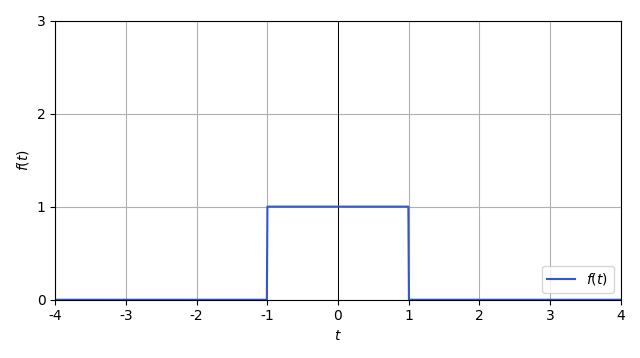
\includegraphics[width=\textwidth]{sources/1_rectangular/graph_1.png}
    \end{minipage}\hfill
    \begin{minipage}{0.5\textwidth}
        \centering 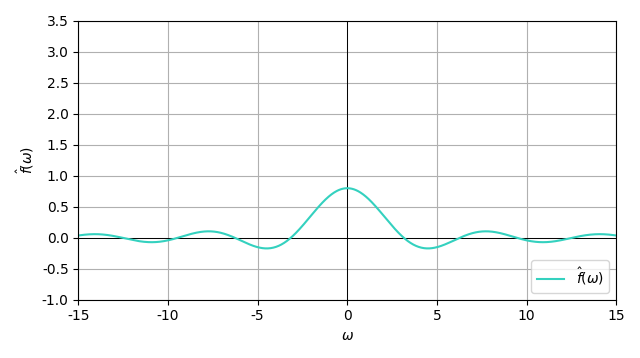
\includegraphics[width=\textwidth]{sources/1_rectangular/fourier_1.png}
    \end{minipage}
    \caption{Графики прямоугольной функции и её Фурье-образа для $a = 1$ и $b = 1$} 
\end{figure}
\begin{figure}[H]
    \begin{minipage}{0.5\textwidth}
        \centering 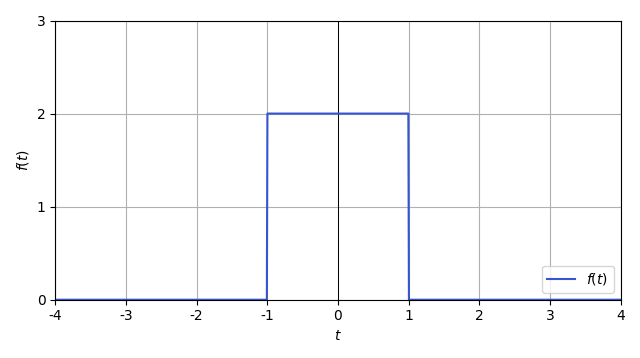
\includegraphics[width=\textwidth]{sources/1_rectangular/graph_2.png}
    \end{minipage}\hfill
    \begin{minipage}{0.5\textwidth}
        \centering 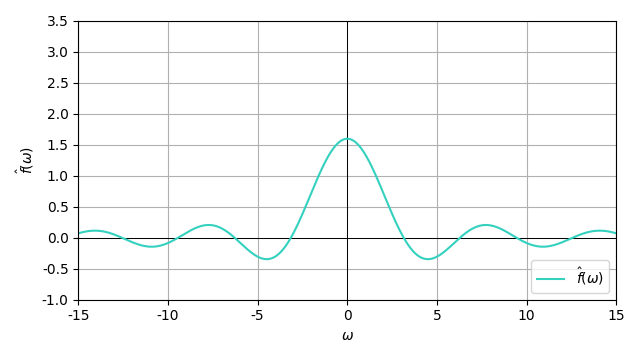
\includegraphics[width=\textwidth]{sources/1_rectangular/fourier_2.png}
    \end{minipage}
    \caption{Графики прямоугольной функции и её Фурье-образа для $a = 2$ и $b = 1$} 
\end{figure}
\begin{figure}[H]
    \begin{minipage}{0.5\textwidth}
        \centering 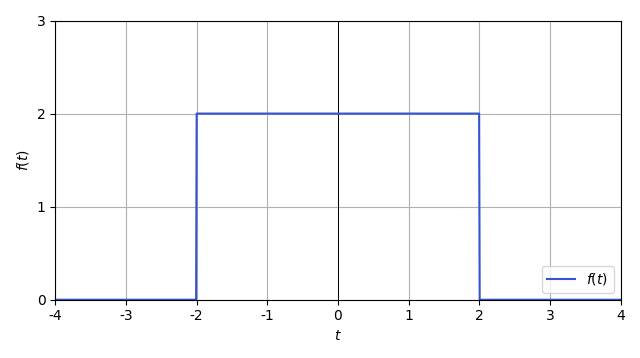
\includegraphics[width=\textwidth]{sources/1_rectangular/graph_3.png}
    \end{minipage}\hfill
    \begin{minipage}{0.5\textwidth}
        \centering 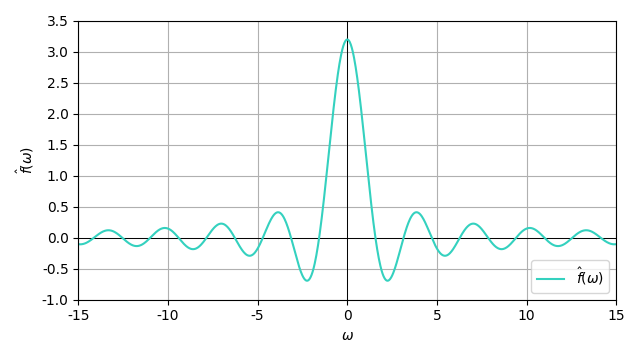
\includegraphics[width=\textwidth]{sources/1_rectangular/fourier_3.png}
    \end{minipage}
    \caption{Графики прямоугольной функции и её Фурье-образа для $a = 2$ и $b = 2$} 
\end{figure}
\noindent Теперь проверим выполнение равенства Парсеваля для каждого из набора параметров $a$ и $b$, использовав модификацию программы с прошлой лаборотной работы.\\
\begin{minipage}{0.33\textwidth}
\begin{lstlisting}[caption={$a = 1$, $b = 1$}]
Parseval deviation:
| ||f||^2 - ||F||^2 | = 0.0063333
\end{lstlisting}
\end{minipage}\hfill
\begin{minipage}{0.33\textwidth}
\begin{lstlisting}[caption={$a = 2$, $b = 1$}, numbers=none]
Parseval deviation:
| ||f||^2 - ||F||^2 | = 0.0253333
\end{lstlisting}
\end{minipage}\hfill
\begin{minipage}{0.33\textwidth}
\begin{lstlisting}[caption={$a = 2$, $b = 2$}, numbers=none]
Parseval deviation:
| ||f||^2 - ||F||^2 | = 0.0253036
\end{lstlisting}
\end{minipage}
Как мы видим, отклонение по равенству Парсеваля совсем небольшое.\\[0.5em]
Чтобы понять, как параметры $a$ и $b$ влияют на исходную функцию и Фурье-образ, достаточно взглянуть на их формулы. В исходной функции $b$ влияет на ширину прямоугольника, а $a$ --- на его высоту. И согласно формуле Фурье-образа, с изменением $a$ изменяется амплитуда кардинального синуса, а изменение $b$ приводит к изменению не только амплитуды, но и частоты. То же самое мы наблюдаем и на графиках.

% MARK: Треугольная функция
\addsubsection{Треугольная функция}
Итак, дана следующая функция, для которой мы будем строить Фурье-образ:
$$f(t) = \begin{cases}
    a - \left|\nicefrac{at}{b}\right|, & \left| t \right| \leqslant b \\
    0, & \left| t \right| > b
\end{cases}
$$
Для начала выведем выражение для вычисление Фурье-образа в общем виде:
$$\hat{f}(\omega)=\frac{1}{\sqrt{2\pi}}\int_{-b}^{b}\left( a - \left| \frac{at}{b} \right| \right)\e^{-i\omega t}dt = \frac{1}{\sqrt{2\pi}}\left( \int_{0}^{b}\left( a - \frac{at}{b} \right)\e^{-i\omega t}dt + \int_{-b}^{0}\left( a + \frac{at}{b} \right)\e^{-i\omega t}dt \right) = $$
$$= \frac{a}{\sqrt{2\pi}}\left( \int_{0}^{b}\left( 1 - \frac{t}{b} \right)\e^{-i\omega t}dt + \int_{-b}^{0}\left( 1 + \frac{t}{b} \right)\e^{-i\omega t}dt\right) = \frac{a}{\sqrt{2\pi}}\left( \frac{(i\omega (t + b) + 1)\e^{-i\omega t}}{b\omega^2}\at^0_{-b} - \frac{(i\omega (t - b) + 1)\e^{-i\omega t}}{b\omega^2}\at^b_0 \right) = $$
$$= \frac{a}{\sqrt{2\pi}}\left( \frac{i\omega b + 1 - \e^{i\omega b}}{b\omega^2} - \frac{\e^{-i\omega b} - 1 + i\omega b}{b\omega^2} \right) = \frac{-a}{\omega^2b\sqrt{2\pi}}\left( \e^{-i\omega b} + \e^{i\omega b} - 2 \right) = \begin{bmatrix}
    \e^{i\omega b} + \e^{-i\omega b} = 2\cos{\omega b}
\end{bmatrix} = $$
$$= \frac{a(2 - 2\cos\omega b)}{\omega^2b\sqrt{2\pi}} = \begin{bmatrix}
    2 - 2\cos{\omega b} = 4\sin^2\nicefrac{\omega b}{2}
\end{bmatrix} = \frac{4a\sin^2{\nicefrac{\omega b}{2}}}{\omega^2 b\sqrt{2\pi}} = \frac{ab}{\sqrt{2\pi}}\text{sinc}^2\,\frac{\omega b}{2}$$
Для каждого из набора коэффициентов формула приобретает следующий вид:
$$\frac{1}{\sqrt{2\pi}}\text{sinc}^2\,\frac{\omega}{2}\text{ для (1, 1)}\qquad\sqrt{\frac{2}{\pi}}\text{sinc}^2\,\frac{\omega}{2}\text{ для (2, 1)}\qquad\sqrt{\frac{8}{\pi}}\text{sinc}^2\,\omega\text{ для (2, 2)}$$
И теперь построим графики исходной функции и её Фурье-образа для каждой из пар значений $(a, b)$, которые мы задали перед выполнением задания.
\begin{figure}[H]
    \begin{minipage}{0.5\textwidth}
        \centering 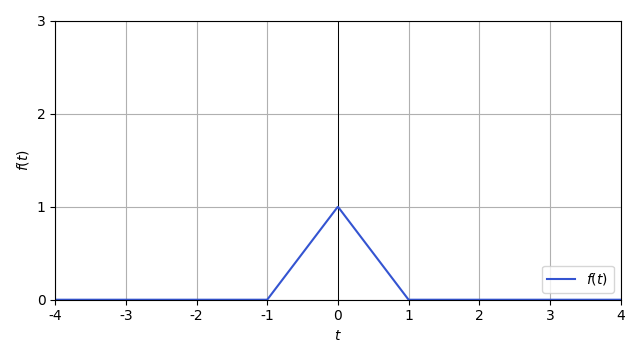
\includegraphics[width=\textwidth]{sources/2_triangular/graph_1.png}
    \end{minipage}\hfill
    \begin{minipage}{0.5\textwidth}
        \centering 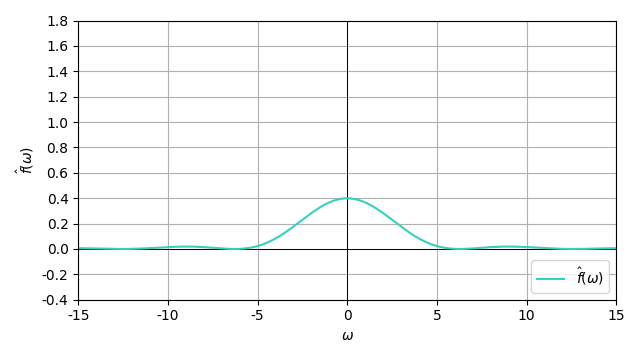
\includegraphics[width=\textwidth]{sources/2_triangular/fourier_1.png}
    \end{minipage}
    \caption{Графики треугольной функции и её Фурье-образа для $a = 1$ и $b = 1$} 
\end{figure}
\begin{figure}[H]
    \begin{minipage}{0.5\textwidth}
        \centering 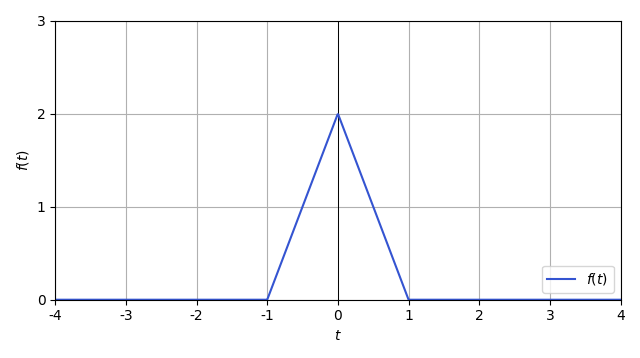
\includegraphics[width=\textwidth]{sources/2_triangular/graph_2.png}
    \end{minipage}\hfill
    \begin{minipage}{0.5\textwidth}
        \centering 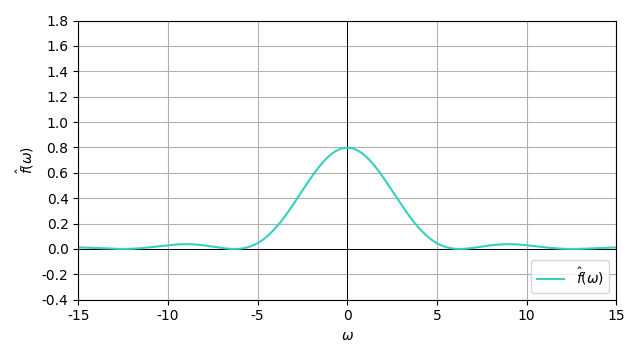
\includegraphics[width=\textwidth]{sources/2_triangular/fourier_2.png}
    \end{minipage}
    \caption{Графики треугольной функции и её Фурье-образа для $a = 2$ и $b = 1$} 
\end{figure}
\begin{figure}[H]
    \begin{minipage}{0.5\textwidth}
        \centering 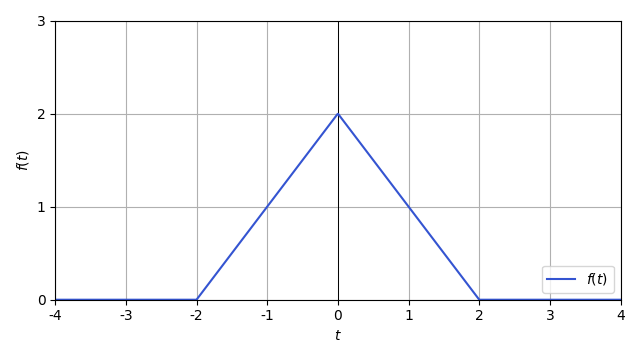
\includegraphics[width=\textwidth]{sources/2_triangular/graph_3.png}
    \end{minipage}\hfill
    \begin{minipage}{0.5\textwidth}
        \centering 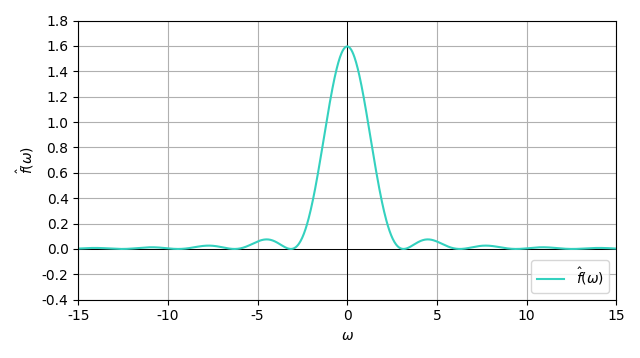
\includegraphics[width=\textwidth]{sources/2_triangular/fourier_3.png}
    \end{minipage}
    \caption{Графики треугольной функции и её Фурье-образа для $a = 2$ и $b = 2$} 
\end{figure}
\noindent Теперь проверим выполнение равенства Парсеваля для каждого из набора параметров $a$ и $b$, использовав модификацию программы с прошлой лаборотной работы.\\
\begin{minipage}{0.33\textwidth}
\begin{lstlisting}[caption={$a = 1$, $b = 1$}]
Parseval deviation:
| ||f||^2 - ||F||^2 | = 0.0000006
\end{lstlisting}
\end{minipage}\hfill
\begin{minipage}{0.33\textwidth}
\begin{lstlisting}[caption={$a = 2$, $b = 1$}, numbers=none]
Parseval deviation:
| ||f||^2 - ||F||^2 | = 0.0000025
\end{lstlisting}
\end{minipage}\hfill
\begin{minipage}{0.33\textwidth}
\begin{lstlisting}[caption={$a = 2$, $b = 2$}, numbers=none]
Parseval deviation:
| ||f||^2 - ||F||^2 | = 0.0000006
\end{lstlisting}
\end{minipage}
При более низкой точности отклонение было бы нулевым, но тем не менее в последних разрядах всё ещё есть цифры ;)\\[0.5em]
В исходной функции $b$ влияет на ширину основания треугольника, а $a$ --- на длину его высоты. И согласно формуле Фурье-образа, с изменением $a$ изменяется амплитуда кардинального синуса, а изменение $b$ приводит к изменению не только амплитуды, но и частоты. То же самое мы наблюдаем и на графиках.

% MARK: Кардинальный синус
\addsubsection{Кардинальный синус}
Итак, перед нами новая функция, для которой мы будем строить Фурье-образ: $f(t) = a\,\text{sinc}\,bt$.\\[0.5em]
Предоставляю результат вычисления Фурье-образа в общем виде, выполненный в Wolfram Alpha:
$$\hat{f}(\omega)=\frac{1}{\sqrt{2\pi}}\int_{-\infty}^{\infty}a\,\text{sinc}(bt)\e^{-i\omega t}dt = \frac{a}{\sqrt{2\pi}}\int_{-\infty}^{\infty}\text{sinc}(bt)\e^{-i\omega t}dt = \frac{a\pi}{\sqrt{2\pi}|b|}\begin{cases}
    0 & \nicefrac{b^2}{\omega^2} \leqslant 1\\ 1 & \text{otherwise}
\end{cases} = \begin{cases}
    0 & -1 \leqslant \nicefrac{b}{\omega} \leqslant 1\\ \sqrt{\dfrac{\pi}{2}}\dfrac{a}{|b|} & \text{otherwise}
\end{cases}$$
И теперь построим графики исходной функции и её Фурье-образа для каждой из пар значений $(a, b)$, которые мы задали перед выполнением задания.
\begin{figure}[H]
    \begin{minipage}{0.5\textwidth}
        \centering 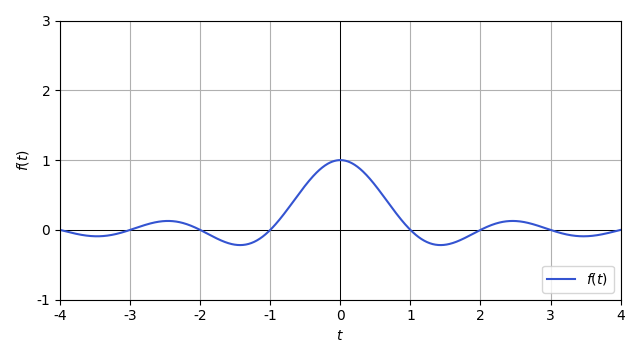
\includegraphics[width=\textwidth]{sources/3_cardinal_sin/graph_1.png}
    \end{minipage}\hfill
    \begin{minipage}{0.5\textwidth}
        \centering 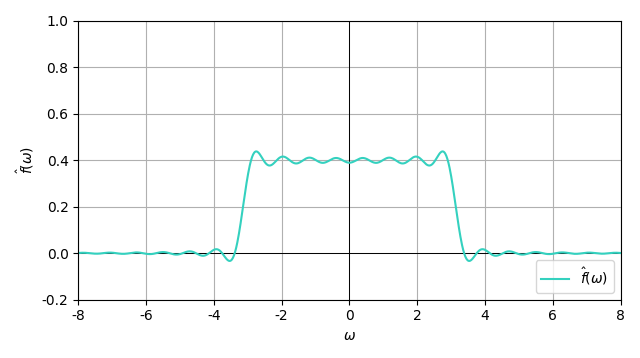
\includegraphics[width=\textwidth]{sources/3_cardinal_sin/fourier_1.png}
    \end{minipage}
    \caption{Графики кардинального синуса и его Фурье-образа для $a = 1$ и $b = 1$} 
\end{figure}
\begin{figure}[H]
    \begin{minipage}{0.5\textwidth}
        \centering 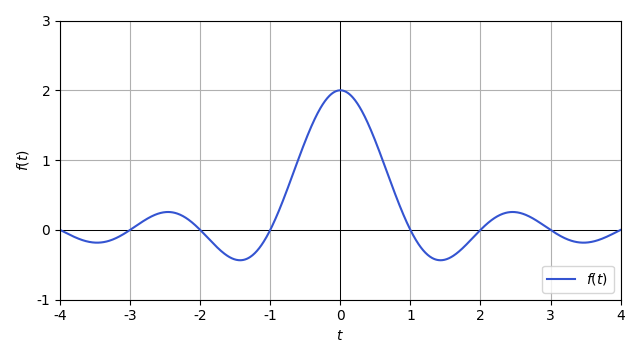
\includegraphics[width=\textwidth]{sources/3_cardinal_sin/graph_2.png}
    \end{minipage}\hfill
    \begin{minipage}{0.5\textwidth}
        \centering 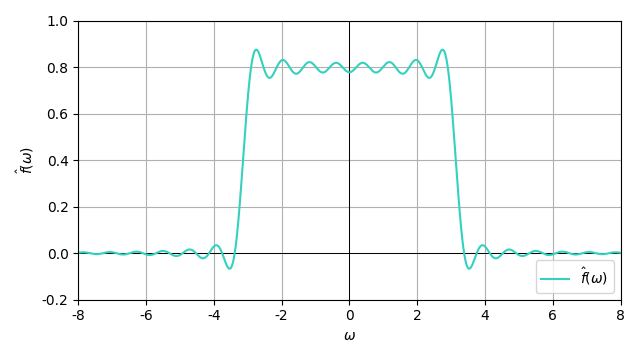
\includegraphics[width=\textwidth]{sources/3_cardinal_sin/fourier_2.png}
    \end{minipage}
    \caption{Графики кардинального синуса и его Фурье-образа для $a = 2$ и $b = 1$} 
\end{figure}
\begin{figure}[H]
    \begin{minipage}{0.5\textwidth}
        \centering 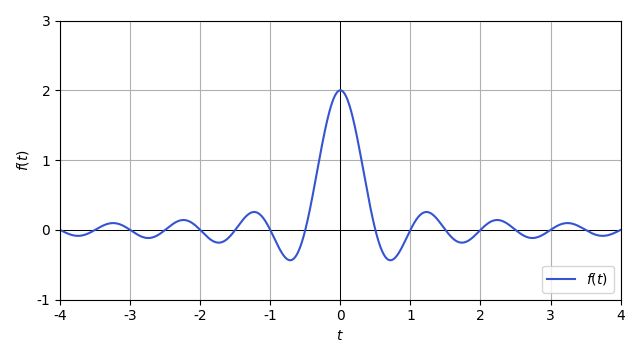
\includegraphics[width=\textwidth]{sources/3_cardinal_sin/graph_3.png}
    \end{minipage}\hfill
    \begin{minipage}{0.5\textwidth}
        \centering 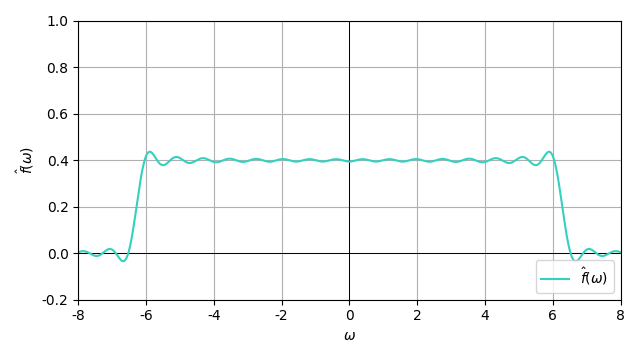
\includegraphics[width=\textwidth]{sources/3_cardinal_sin/fourier_3.png}
    \end{minipage}
    \caption{Графики кардинального синуса и его Фурье-образа для $a = 2$ и $b = 2$} 
\end{figure}
\noindent Теперь проверим выполнение равенства Парсеваля для каждого из набора параметров $a$ и $b$, использовав модификацию программы с прошлой лаборотной работы.\\
\begin{minipage}{0.33\textwidth}
\begin{lstlisting}[caption={$a = 1$, $b = 1$}]
Parseval deviation:
| ||f||^2 - ||F||^2 | = 0.0000002
\end{lstlisting}
\end{minipage}\hfill
\begin{minipage}{0.33\textwidth}
\begin{lstlisting}[caption={$a = 2$, $b = 1$}, numbers=none]
Parseval deviation:
| ||f||^2 - ||F||^2 | = 0.0000009
\end{lstlisting}
\end{minipage}\hfill
\begin{minipage}{0.33\textwidth}
\begin{lstlisting}[caption={$a = 2$, $b = 2$}, numbers=none]
Parseval deviation:
| ||f||^2 - ||F||^2 | = 0.0000002
\end{lstlisting}
\end{minipage}
И, опять же, наблюдаем практически полное отсутствие отклонение по равенству Парсеваля.\\[0.5em]
Говоря о влиянии параметров $a$ и $b$ на вид исходной функции и Фурье-образа: параметр $a$ прямо пропорционально влияет на амплитуду обеих функций, а параметр $b$ прямо пропорционально влияет на частоту исходной функции и на ширину приподнятого участка Фурье-образа, а также обратно пропорционально влияет на амплитуду Фурье-образа. И, что примечательно, частота второй гармоники Фурье-образа остаётся неизменной. То же самое мы наблюдаем и на графиках.

% MARK: Функция Гаусса
\addsubsection{Функция Гаусса}
А теперь мы будем строить Фурье-образ для функции Гаусса: $f(t) = a\e^{-bt^2}$.\\[0.5em]
Предоставляю результат вычисления Фурье-образа в общем виде, выполненный в Wolfram Alpha:
$$\hat{f}(\omega)=\frac{1}{\sqrt{2\pi}}\int_{-\infty}^{\infty}a\e^{-bt^2}\e^{-i\omega t}dt = \frac{a}{\sqrt{2\pi}}\int_{-\infty}^{\infty}\e^{-bt^2-i\omega t}dt = \frac{a\sqrt{\pi}\e^{\nicefrac{-w^2}{4b}}}{\sqrt{2\pi b}} = \frac{a\e^{\nicefrac{-w^2}{4b}}}{\sqrt{2b}}$$
Для каждого из набора коэффициентов формула приобретает следующий вид:
$$\frac{\e^{\nicefrac{-w^2}{4}}}{\sqrt{2}}\text{ для (1, 1)}\qquad\sqrt{2}\e^{\nicefrac{-w^2}{4}}\text{ для (2, 1)}\qquad\e^{\nicefrac{-w^2}{8}}\text{ для (2, 2)}$$
Пришло время строить графики исходной функции и её Фурье-образа для каждой из пар значений $(a, b)$, которые мы задали перед выполнением задания.
\begin{figure}[H]
    \begin{minipage}{0.5\textwidth}
        \centering 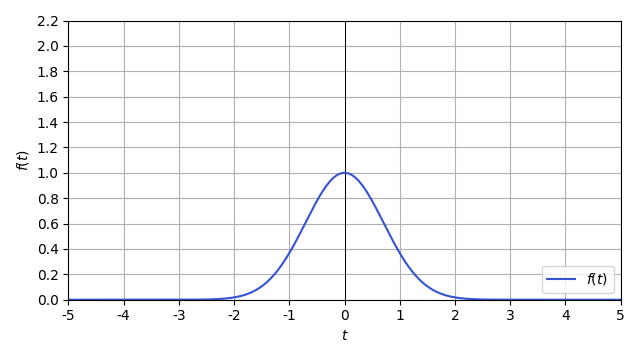
\includegraphics[width=\textwidth]{sources/4_gaussian/graph_1.png}
    \end{minipage}\hfill
    \begin{minipage}{0.5\textwidth}
        \centering 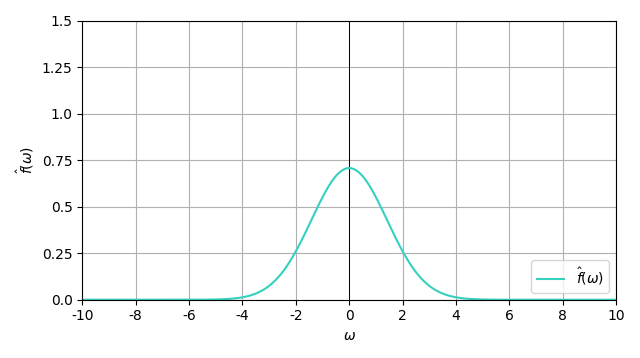
\includegraphics[width=\textwidth]{sources/4_gaussian/fourier_1.png}
    \end{minipage}
    \caption{Графики функции Гаусса и её Фурье-образа для $a = 1$ и $b = 1$} 
\end{figure}
\begin{figure}[H]
    \begin{minipage}{0.5\textwidth}
        \centering 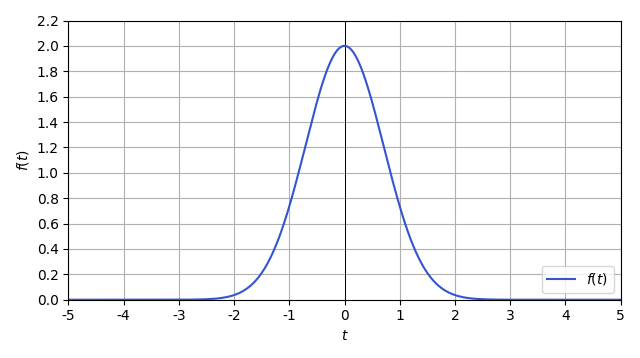
\includegraphics[width=\textwidth]{sources/4_gaussian/graph_2.png}
    \end{minipage}\hfill
    \begin{minipage}{0.5\textwidth}
        \centering 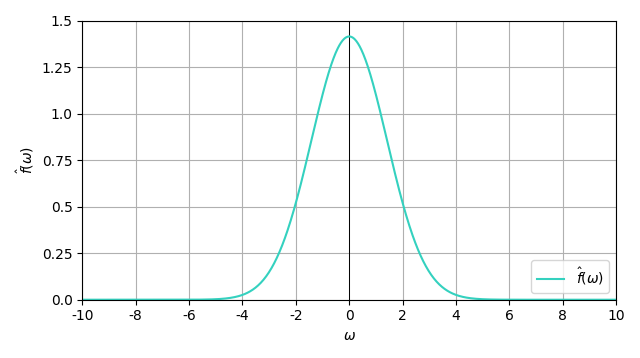
\includegraphics[width=\textwidth]{sources/4_gaussian/fourier_2.png}
    \end{minipage}
    \caption{Графики функции Гаусса и её Фурье-образа для $a = 2$ и $b = 1$} 
\end{figure}
\begin{figure}[H]
    \begin{minipage}{0.5\textwidth}
        \centering 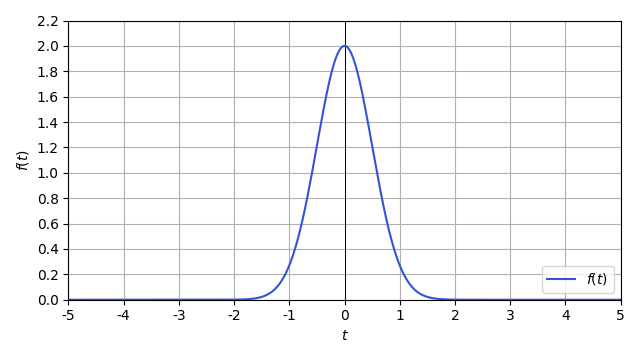
\includegraphics[width=\textwidth]{sources/4_gaussian/graph_3.png}
    \end{minipage}\hfill
    \begin{minipage}{0.5\textwidth}
        \centering 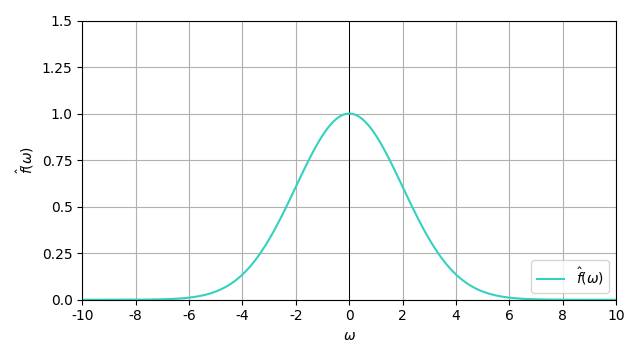
\includegraphics[width=\textwidth]{sources/4_gaussian/fourier_3.png}
    \end{minipage}
    \caption{Графики функции Гаусса и её Фурье-образа для $a = 2$ и $b = 2$} 
\end{figure}
\noindent Теперь проверим выполнение равенства Парсеваля для каждого из набора параметров $a$ и $b$, использовав модификацию программы с прошлой лаборотной работы.\\
\begin{minipage}{0.33\textwidth}
\begin{lstlisting}[caption={$a = 1$, $b = 1$}]
Parseval deviation:
| ||f||^2 - ||F||^2 | = 0.0008553
\end{lstlisting}
\end{minipage}\hfill
\begin{minipage}{0.33\textwidth}
\begin{lstlisting}[caption={$a = 2$, $b = 1$}, numbers=none]
Parseval deviation:
| ||f||^2 - ||F||^2 | = 0.0034212
\end{lstlisting}
\end{minipage}\hfill
\begin{minipage}{0.33\textwidth}
\begin{lstlisting}[caption={$a = 2$, $b = 2$}, numbers=none]
Parseval deviation:
| ||f||^2 - ||F||^2 | = 0.0000000
\end{lstlisting}
\end{minipage}
Наблюдаем низкое отклонение по равенству Парсеваля, что говорит о хорошем приближении Фурье-образа к исходной функции.\\[0.5em]
В исходной функции $b$ обратно пропоционально влияет на её ширину, а $a$ влияет прямо пропоционально на амплитуду. Для Фурье-образа с увеличением $a$ растёт амплитуда, а изменение $b$ прямо пропорционально изменяет её ширину и обратно пропорционально изменяет её амплитуду. То же самое мы наблюдаем и на графиках.

% MARK: Двустороннее затухание
\addsubsection{Двустороннее затухание}
И перед нами последняя функция из тех, для которых строится вещественный Фурье-образ: $f(t) = a\e^{-b|t|}$.\\[0.5em]
Для начала выведем выражение для вычисление Фурье-образа в общем виде:
$$\hat{f}(\omega)=\frac{1}{\sqrt{2\pi}}\int_{-\infty}^{\infty}a\e^{-b|t|}\e^{-i\omega t}dt = \frac{a}{\sqrt{2\pi}}\int_{-\infty}^{\infty}\e^{-b|t|-i\omega t}dt = \frac{a}{\sqrt{2\pi}}\left( \int_{0}^{\infty}\e^{-t(b+i\omega)}dt + \int_{-\infty}^{0}\e^{t(b-i\omega)}dt \right) = $$
$$= \frac{a}{\sqrt{2\pi}}\left( \frac{e^{t(b-i\omega)}}{b - i\omega}\at^0_{-\infty} + \frac{e^{-t(b + i\omega)}}{b + i\omega}\at^0_\infty \right) = \frac{a}{\sqrt{2\pi}}\left( \frac{1}{b - i\omega} - \cancel{\frac{e^{-\infty(b-i\omega)}}{b - i\omega}} + \frac{1}{b+i\omega} - \cancel{\frac{e^{-\infty(b+i\omega)}}{b+i\omega}} \right) = $$
$$= \frac{a}{\sqrt{2\pi}}\left( \frac{1}{b-i\omega} + \frac{1}{b+i\omega} \right) = \frac{2ab}{\sqrt{2\pi}(b^2 + \omega^2)} = \frac{ab}{(b^2+\omega^2)}\sqrt{\frac{2}{\pi}}$$
И теперь построим графики исходной функции и её Фурье-образа для каждой из пар значений $(a, b)$, которые мы задали перед выполнением задания.
\begin{figure}[H]
    \begin{minipage}{0.5\textwidth}
        \centering 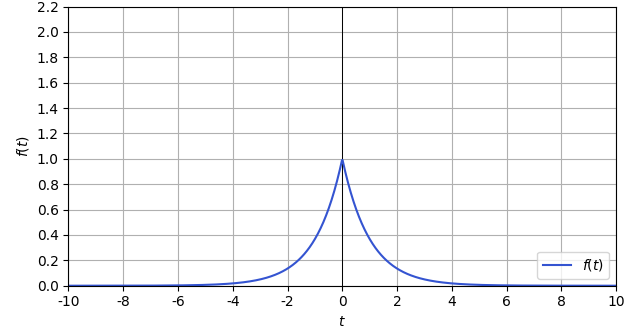
\includegraphics[width=\textwidth]{sources/5_fade/graph_1.png}
    \end{minipage}\hfill
    \begin{minipage}{0.5\textwidth}
        \centering 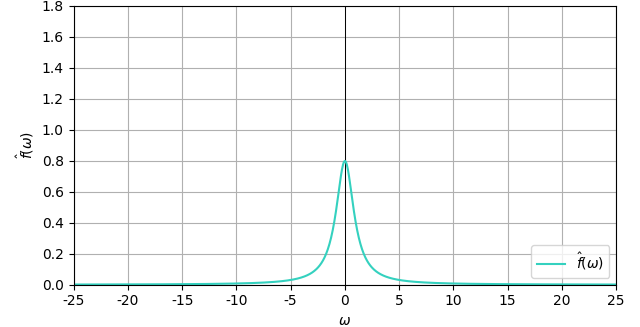
\includegraphics[width=\textwidth]{sources/5_fade/fourier_1.png}
    \end{minipage}
    \caption{Графики двустороннего затухания и его Фурье-образа для $a = 1$ и $b = 1$} 
\end{figure}
\begin{figure}[H]
    \begin{minipage}{0.5\textwidth}
        \centering 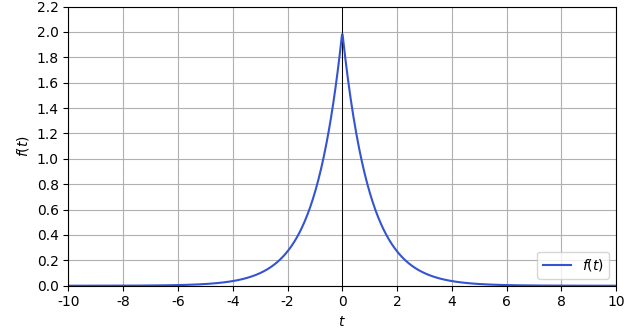
\includegraphics[width=\textwidth]{sources/5_fade/graph_2.png}
    \end{minipage}\hfill
    \begin{minipage}{0.5\textwidth}
        \centering 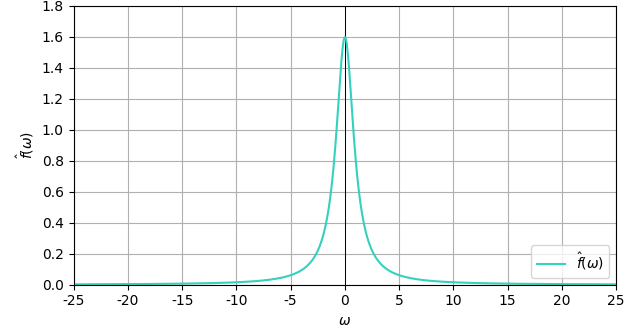
\includegraphics[width=\textwidth]{sources/5_fade/fourier_2.png}
    \end{minipage}
    \caption{Графики двустороннего затухания и его Фурье-образа для $a = 2$ и $b = 1$} 
\end{figure}
\begin{figure}[H]
    \begin{minipage}{0.5\textwidth}
        \centering 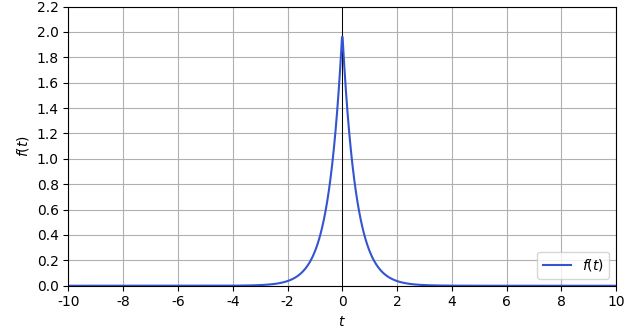
\includegraphics[width=\textwidth]{sources/5_fade/graph_3.png}
    \end{minipage}\hfill
    \begin{minipage}{0.5\textwidth}
        \centering 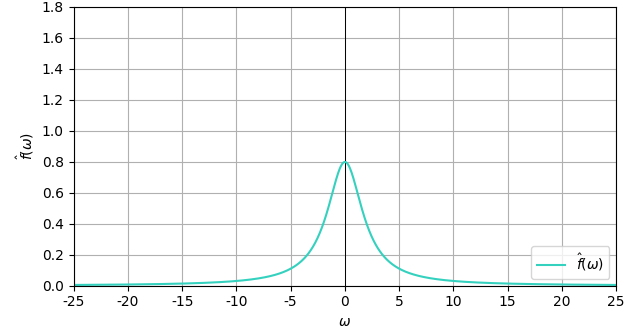
\includegraphics[width=\textwidth]{sources/5_fade/fourier_3.png}
    \end{minipage}
    \caption{Графики двустороннего затухания и его Фурье-образа для $a = 2$ и $b = 2$} 
\end{figure}
\noindent Теперь проверим выполнение равенства Парсеваля для каждого из набора параметров $a$ и $b$, использовав модификацию программы с прошлой лаборотной работы.\\
\begin{minipage}{0.33\textwidth}
\begin{lstlisting}[caption={$a = 1$, $b = 1$}]
Parseval deviation:
| ||f||^2 - ||F||^2 | = 0.0008574
\end{lstlisting}
\end{minipage}\hfill
\begin{minipage}{0.33\textwidth}
\begin{lstlisting}[caption={$a = 2$, $b = 1$}, numbers=none]
Parseval deviation:
| ||f||^2 - ||F||^2 | = 0.0034297
\end{lstlisting}
\end{minipage}\hfill
\begin{minipage}{0.33\textwidth}
\begin{lstlisting}[caption={$a = 2$, $b = 2$}, numbers=none]
Parseval deviation:
| ||f||^2 - ||F||^2 | = 0.0000153
\end{lstlisting}
\end{minipage}
И вновь перед нами низкое отклонение по равенству Парсеваля, что говорит о хорошем приближении Фурье-образа к исходной функции.\\[0.5em]
В исходной функции $b$ влияет на ширину основания треугольника, а $a$ --- на длину его высоты. И согласно формуле Фурье-образа, с изменением $a$ изменяется амплитуда кардинального синуса, а изменение $b$ приводит к изменению не только амплитуды, но и частоты. То же самое мы наблюдаем и на графиках.

% MARK: Задание №2
\addsection{Задание №2. Комплексное преобразование}
В этом задании, как и в предыдущем, нам понадобится унитарное преобразование Фурье к уголовой частоте. Мы будем сдвигать треугольную функцию вправо и влево --- для этого возьмём два положительных и два отрицательных коэффициента $c = \{-5, -2, 3, 4\}$. И зафиксируем у треугольной функции $a = 1$ и $b = 2$. Тогда функция к рассмотрению следующая:
$$f(t) = \begin{cases}
    1 - \left|\nicefrac{t}{2}\right|, & \left| t \right| \leqslant 2 \\
    0, & \left| t \right| > 2
\end{cases}
$$
Определим функцию $g(t) = f(t + c)$. Тогда с учётом выше заданного набора $c$ она приобретает такой вид:
$$g(t) = \begin{cases}
    1 - \left|\frac{t - 5}{2}\right|, & \left| t - 5 \right| \leqslant 2 \\
    0, & \left| t - 5 \right| > 2 
\end{cases}\text{ для }c=-5\qquad
g(t) = \begin{cases}
    1 - \left|\frac{t - 2}{2}\right|, & \left| t - 2 \right| \leqslant 2 \\
    0, & \left| t - 2 \right| > 2 
\end{cases}\text{ для }c=-2$$
$$g(t) = \begin{cases}
    1 - \left|\frac{t + 3}{2}\right|, & \left| t + 3 \right| \leqslant 2 \\
    0, & \left| t + 3 \right| > 2 
\end{cases}\text{ для }c=3\qquad
g(t) = \begin{cases}
    1 - \left|\frac{t + 4}{2}\right|, & \left| t + 4 \right| \leqslant 2 \\
    0, & \left| t + 4 \right| > 2
\end{cases}\text{ для }c=4
$$
Но преобразовывать функцию к Фурье-образу мы будем в общем виде $f(t + c)$ и только затем уже подставлять конкретные значения $c$:
$$\hat{g}(\omega)=\frac{1}{\sqrt{2\pi}}\int_{-2}^{2}\left( 1 - \left| \frac{t + c}{2} \right| \right)\e^{-i\omega t}dt=\frac{1}{\sqrt{2\pi}}\int_{-2}^{2}\left( 1 - \left| \frac{t}{2} \right| \right)\e^{-i\omega (t - c)}dt = $$
$$ = \frac{1}{\sqrt{2\pi}}\left( \int_{0}^{2}\left( 1 - \frac{t}{2} \right)\e^{-i\omega (t - c)}dt + \int_{-2}^{0}\left( 1 + \frac{t}{2} \right)\e^{-i\omega (t - c)}dt \right) = \frac{1}{\sqrt{2\pi}}\left( \frac{(i\omega (t + 2) + 1)\e^{i\omega(c-t)}}{2\omega^2}\at^0_{-2} -\right.$$
$$\left. - \frac{(i\omega (t - 2) + 1)\e^{i\omega(c-t)}}{2\omega^2}\at^2_0 \right) = \frac{1}{\sqrt{2\pi}}\left( \frac{2\e^{i\omega c} - \e^{i\omega(c-2)} - \e^{i\omega(c+2)}}{2\omega^2} \right) = \frac{-\e^{i\omega c}}{2\omega^2\sqrt{2\pi}}\left( \e^{-2i\omega} + \e^{2i\omega} - 2 \right) = $$
$$ = \begin{bmatrix}
    \e^{2i\omega} + \e^{-2i\omega} = 2\cos{2\omega}
\end{bmatrix} = \frac{\e^{i\omega c}(2 - 2\cos2\omega)}{2\omega^2\sqrt{2\pi}} = \begin{bmatrix}
    2 - 2\cos{2\omega} = 4\sin^2\omega
\end{bmatrix} = \frac{4\e^{i\omega c}\sin^2\omega}{2\omega^2\sqrt{2\pi}} = \frac{2e^{i\omega c}}{\sqrt{2\pi}}\text{sinc}^2\,\omega$$
Сравнивая с Фурье-образом треугольной функции без сдвигов при тех же коэффициентах выясняем, что разница между $\hat{f}(\omega)$ и $\hat{g}(\omega)$ в множителе $e^{i\omega c}$, который как раз и придаёт Фурье-образу комплексные свойства.\\[0.5em]
Рассмотрим графики функции $g(t)$ с разными сдвигами:
\begin{figure}[H]
    \begin{minipage}{0.5\textwidth}
        \centering 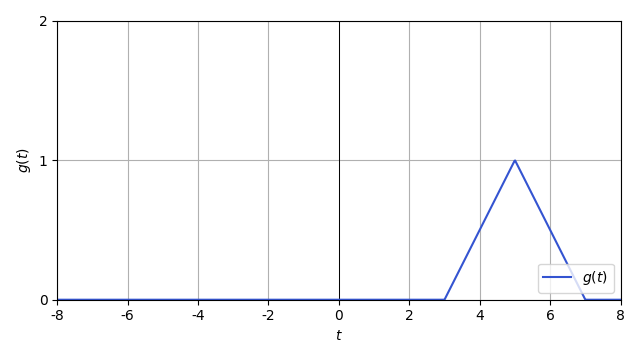
\includegraphics[width=\textwidth]{sources/6_complex/graph_1.png}
        \caption{График функции $g(t)$ со сдвигом $c = -5$} 
    \end{minipage}\hfill
    \begin{minipage}{0.5\textwidth}
        \centering 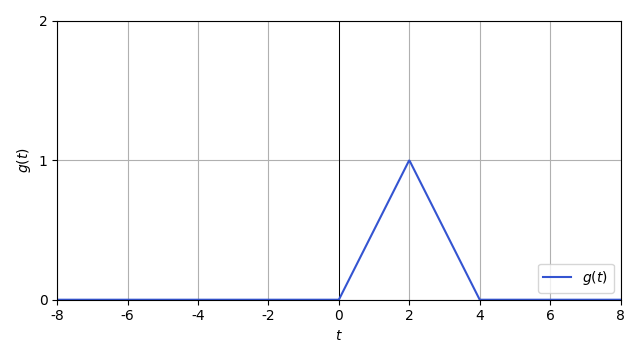
\includegraphics[width=\textwidth]{sources/6_complex/graph_2.png}
        \caption{График функции $g(t)$ со сдвигом $c = -2$} 
    \end{minipage}
\end{figure}
\begin{figure}[H]
    \begin{minipage}{0.5\textwidth}
        \centering 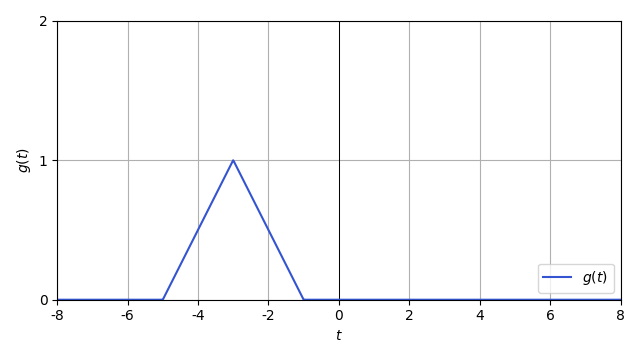
\includegraphics[width=\textwidth]{sources/6_complex/graph_3.png}
        \caption{График функции $g(t)$ со сдвигом $c = 3$} 
    \end{minipage}\hfill
    \begin{minipage}{0.5\textwidth}
        \centering 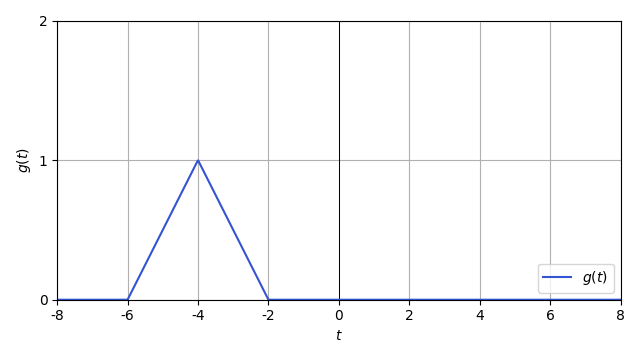
\includegraphics[width=\textwidth]{sources/6_complex/graph_4.png}
        \caption{График функции $g(t)$ со сдвигом $c = 4$} 
    \end{minipage}
\end{figure}
\noindent И теперь построим для каждого из сдвигов $c$ графики с действительной и мнимой частями Фурье-образа и модулем Фурье-образа.
\begin{figure}[H]
    \begin{minipage}{0.5\textwidth}
        \centering 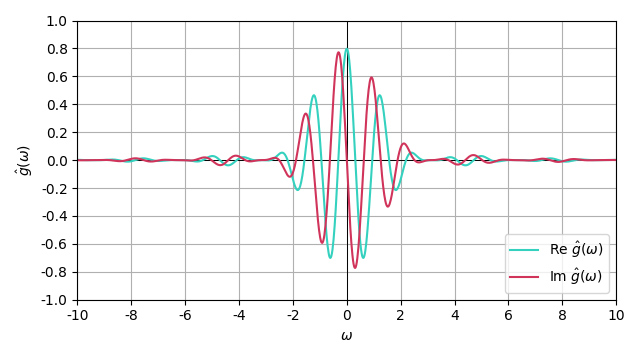
\includegraphics[width=\textwidth]{sources/6_complex/fourier_1.png}
    \end{minipage}\hfill
    \begin{minipage}{0.5\textwidth}
        \centering 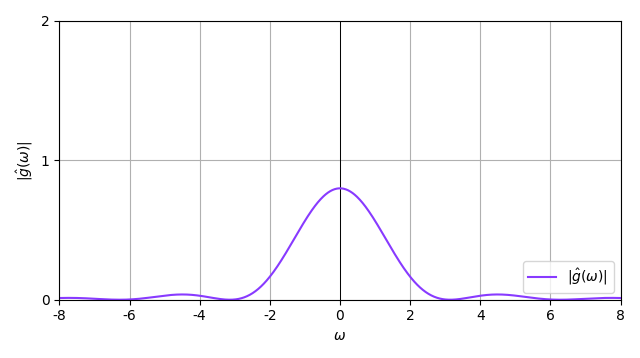
\includegraphics[width=\textwidth]{sources/6_complex/abs_1.png}
    \end{minipage}
    \caption{Графики Фурье-образа для исходной функции со сдвигом $c = -5$} 
\end{figure}
\begin{figure}[H]
    \begin{minipage}{0.5\textwidth}
        \centering 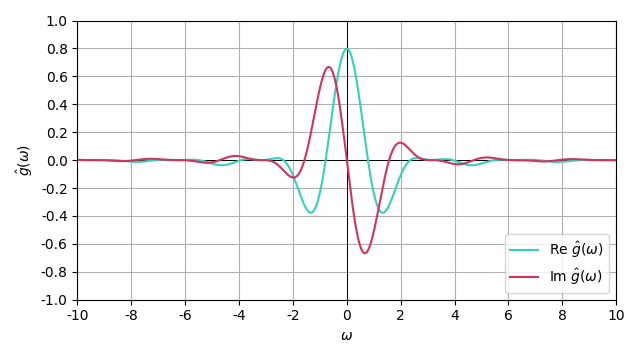
\includegraphics[width=\textwidth]{sources/6_complex/fourier_2.png}
    \end{minipage}\hfill
    \begin{minipage}{0.5\textwidth}
        \centering 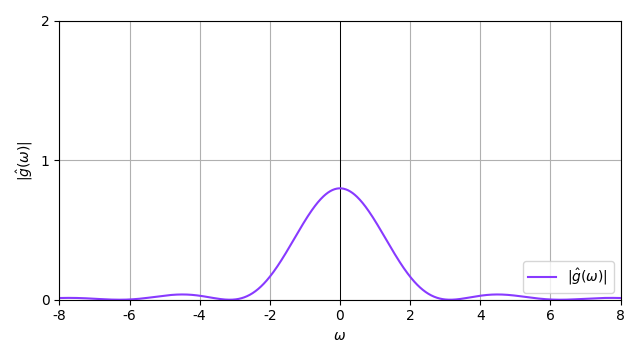
\includegraphics[width=\textwidth]{sources/6_complex/abs_2.png}
    \end{minipage}
    \caption{Графики Фурье-образа для исходной функции со сдвигом $c = -2$} 
\end{figure}
\begin{figure}[H]
    \begin{minipage}{0.5\textwidth}
        \centering 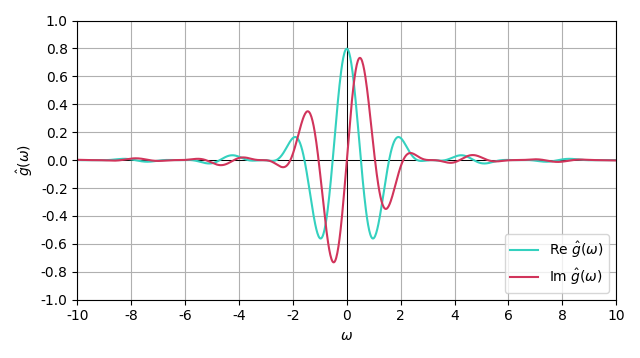
\includegraphics[width=\textwidth]{sources/6_complex/fourier_3.png}
    \end{minipage}\hfill
    \begin{minipage}{0.5\textwidth}
        \centering 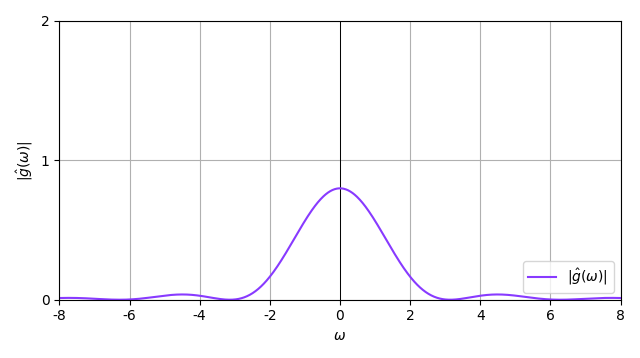
\includegraphics[width=\textwidth]{sources/6_complex/abs_3.png}
    \end{minipage}
    \caption{Графики Фурье-образа для исходной функции со сдвигом $c = 3$} 
\end{figure}
\begin{figure}[H]
    \begin{minipage}{0.5\textwidth}
        \centering 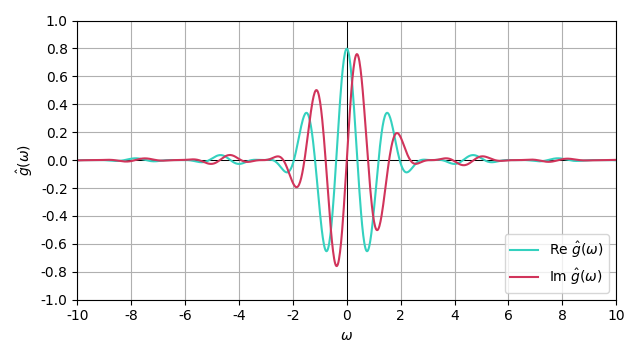
\includegraphics[width=\textwidth]{sources/6_complex/fourier_4.png}
    \end{minipage}\hfill
    \begin{minipage}{0.5\textwidth}
        \centering 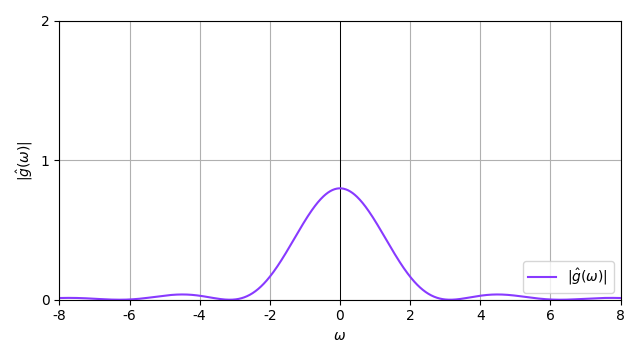
\includegraphics[width=\textwidth]{sources/6_complex/abs_4.png}
    \end{minipage}
    \caption{Графики Фурье-образа для исходной функции со сдвигом $c = 4$} 
\end{figure}
\noindent Как мы видим, амплитуды действительной и мнимой части Фурье-образа остаются неизменными, а вот чем больше $|c|$, тем выше частота $\text{Re}\,\hat{g}(\omega)$ и $\text{Im}\,\hat{g}(\omega)$. В зависимости от знака коэффициента $c$ мнимая часть Фурье-образа находится либо справа ($c > 0$), либо слева ($c < 0$) от оси ординат. Вещественная часть Фурье-образа при этом симметрична относительно оси ординат.\\[0.5em]
Обратим внимание на модуль Фурье-образа. Он равен при всех сдвигах исходной функции и похож на вещественный Фурье-образ функции, как если бы она не была сдвинута.
% MARK: Задание №3
\addsection{Задание №3. Музыкальное преобразование}
Перед началом выполнения задания обозначим унитарное преобразование Фурье к обычной частоте $\nu$:
$$\hat{f}(\nu) = \int_{-\infty}^{\infty}f(t)\e^{-2\pi i\nu t}\,dt\qquad\leftrightarrows\qquad f(t) = \int_{-\infty}^{\infty}\hat{f}(\nu)\e^{2\pi i\nu t}\,d\nu\ \ \text{(обратное преобразование)}$$
Для обработки я выбрал аккорд №2 и с помощью библиотеки \verb|librosa| в \textbf{Python} я преобразовал сигнал из аудиофайла в набор амплитуд, которые мы теперь можем проанализировать.\\[0.5em]
В целях упрощения работы с аудиофайлом, в нём предварительно была вырезана лишняя тишина в начале и в конце, а также аудиодорожка была нормализована, чтобы общий уровень громкости поднялся.\\[0.5em]
Теперь посмотрим на график зависимости времени от амплитуды:
\begin{figure}[H]
    \centering 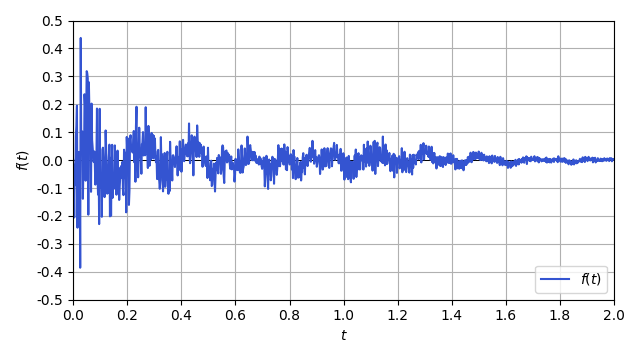
\includegraphics[width=0.7\textwidth]{sources/7_accord/graph.png}
    \caption{График зависимости амплитуды от времени} 
\end{figure}
\noindent Ну что ж, применим преобразование Фурье к нашему аудиосигналу и посмотрим на модуль получившегося Фурье-образа:
\begin{figure}[H]
    \centering 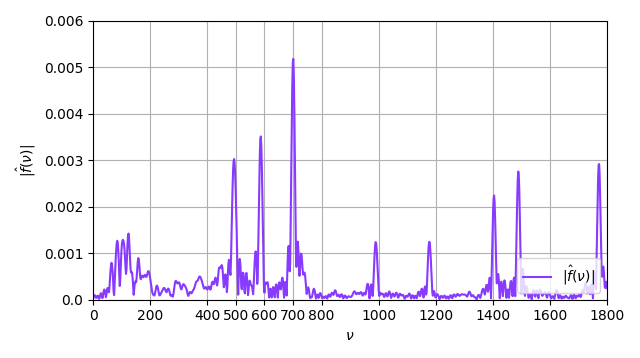
\includegraphics[width=0.7\textwidth]{sources/7_accord/abs.png}
    \caption{Модуль Фурье-образа аудиосигнала}
\end{figure}
\noindent На графике я выделил, что на частотах, близких к 500, 600 и 700 Гц находятся пики, которые вероятнее всего определяют аккорд. Уточняем частоты по таблице частот и нот: B4 на частоте 493.88 Гц, D5 на частоте 587.32 Гц и F5 на частоте 698.46 Гц --- именно из таких нот состоит аккорд. Убедиться в этом можно, прослушав \href{https://drive.google.com/file/d/1BIB_1OWBz3JtAMP4OqDv1_yxtRN3A89a/view}{мою запись} каждой из трёх нот по отдельности. И, если мне не изменяет память, это \underline{трезвучие Bdim}.
\end{document}